% !TEX root=../../thesis.tex

\section{Prototype functionality} % (fold)
\label{sec:prototype_functionality}
As part of answering the research question, a prototype was developed. In this
section we will describe the functionality in the prototype.\\

The prototype is a map based system that presents the information according to
the needs of the stakeholders, we present the system in
\Ref{fig:map_prototype}. The system uses the 



\begin{figure}[!htbp]
	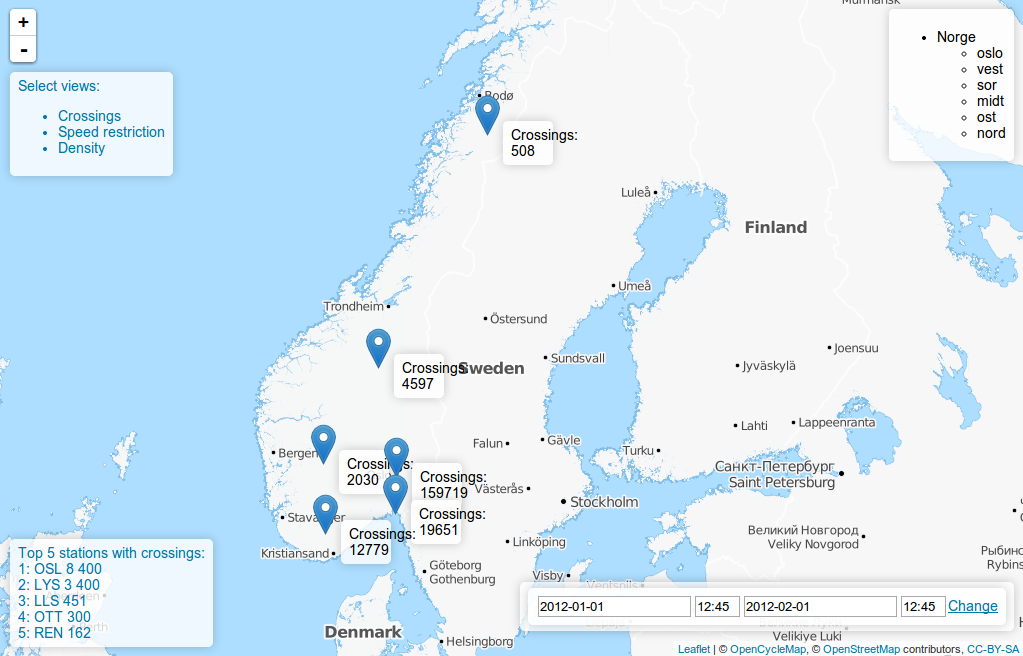
\includegraphics[width=\textwidth,center]{map_prototype.png}
	\caption[Map implementation]{Map implementation}
	\label{fig:map_prototype}
\end{figure}

\begin{figure}[h!tbp]
	\centering
	\begin{subfigure}{0.4\textwidth}
		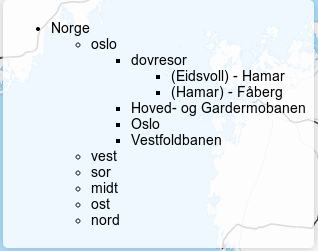
\includegraphics[width=\textwidth]{stakeholder_selection_list.png}
		\caption[Stakeholder selection list]{Stakeholder selection list}
		\label{fig:stakeholder_selection_list}
	\end{subfigure}
	\begin{subfigure}{0.3\textwidth}
		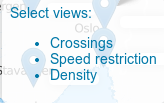
\includegraphics[width=\textwidth]{information_type_selection.png}
		\caption[Information type selection]{Information type selection}
		\label{fig:implementation_type_selection}
	\end{subfigure}
	\caption[Stakeholder selection and Information type]{Stakeholder selection and Information type}
	\label{fig:stakeholder_selection_and_information_type}
\end{figure}

\begin{figure}[h!tbp]
	\centering
	\begin{subfigure}{0.4\textwidth}
		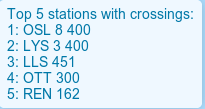
\includegraphics[width=\textwidth]{top5.png}
		\caption[Top 5 list]{Top 5 list}
		\label{fig:top_5_list}
	\end{subfigure}
	\begin{subfigure}{0.6\textwidth}
		
\includegraphics[width=\textwidth]{time_selection_implemented.png}
		\caption[Time selection implementation]{Time selection implementation}
		\label{fig:time_selection_implemented}
	\end{subfigure}
	\caption[Top 5 list and Time selection]{Top 5 list and Time selection}
	\label{fig:Top5_list_and_time_selection}
\end{figure}

\begin{figure}[h!tbp]
	\centering
	\begin{subfigure}{0.6\textwidth}
		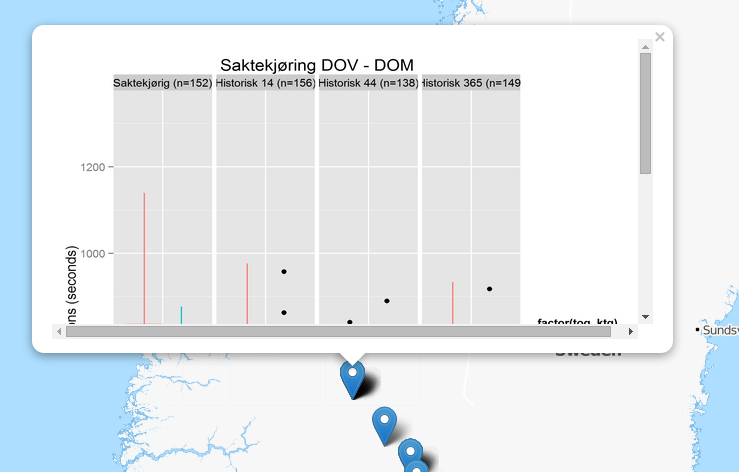
\includegraphics[width=\textwidth]{speed_restriction_presentation.png}
		\caption[Speed restriction presentation]{Speed restriction presentation}
		\label{fig:speed_restriction_presentation}
	\end{subfigure}
	\begin{subfigure}{0.25\textwidth}
		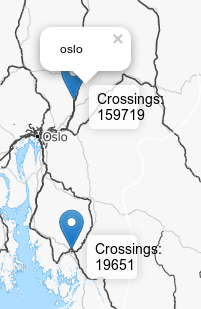
\includegraphics[width=\textwidth]{crossings_presentation.png}
		\caption[Crossings presentation]{Crossings presentation}
		\label{fig:crossings_presentation}
	\end{subfigure}
	\caption[Speed restriction and Crossings implementation]{Speed restriction and Crossings implementation}
	\label{fig:crossings_and_speed_restriction_implementation}
\end{figure}

% section prototype_functionality (end)
